\documentclass[a4paper,10pt,twocolumn]{article}
\usepackage{cite}
\usepackage{listings}
\usepackage[english]{babel}
\usepackage[T1]{fontenc}
\usepackage{amsmath}
\usepackage{amssymb}
\usepackage{graphicx}
\usepackage[]{circuitikz}
\setlength{\oddsidemargin}{0in}
\setlength{\topmargin}{-.8in}
\setlength{\textheight}{9.7in} \setlength{\textwidth}{6.5in}
\usepackage{color,hyperref}
\definecolor{darkblue}{rgb}{0.0,0.0,0.3}
\hypersetup{colorlinks,breaklinks,
            linkcolor=darkblue,urlcolor=darkblue,
            anchorcolor=darkblue,citecolor=darkblue}
\providecommand*\url[1]{\href{#1}{#1}}
\renewcommand*\url[1]{\href{#1}{\texttt{#1}}}

\newcommand{\bm}[1]{\boldsymbol{#1}}
\newcommand{\bh}[1]{\boldsymbol{\hat{#1}}}
\newcommand{\bt}[1]{\boldsymbol{\tilde{#1}}}
\newcommand{\bbar}[1]{\boldsymbol{\bar{#1}}}
\newcommand{\mbf}[1]{\ensuremath{\mathbf{#1}}}
\newcommand{\ode}[2]{\ensuremath{\frac{\mathrm{d} #1}{\mathrm{d} #2}}}
\newcommand{\odet}[2]{\ensuremath{\tfrac{\mathrm{d} #1}{\mathrm{d} #2}}}
\newcommand{\oden}[3]{\ensuremath{\frac{\mathrm{d}^#3 #1}{\mathrm{d} #2^#3}}}
\newcommand{\pde}[2]{\ensuremath{\frac{\partial #1}{\partial #2}}}
\newcommand{\pdet}[2]{\ensuremath{\tfrac{\partial #1}{\partial #2}}}
\newcommand{\pden}[3]{\ensuremath{\frac{\partial^{#3} #1}{\partial
      #2^{#3}}}}
\newcommand{\sub}[1]{\ensuremath{_{\rm{#1}}}}
\newcommand{\arriba}[1]{\ensuremath{^{\rm{#1}}}}
%
\newcommand{\N}{\ensuremath{\mathbb{N}}}
\newcommand{\R}{\ensuremath{\mathbb{R}}}
\newcommand{\C}{\ensuremath{\mathbb{C}}}
\newcommand{\ee}[1]{\ensuremath{\mathrm{e}^{#1}}}
\newcommand{\hdos}{\ensuremath{\mathrm{H}_2}}
\newcommand{\COdos}{\ensuremath{\mathrm{CO}_2}}
\newcommand{\ATP}{\ensuremath{\mathrm{ATP}}}

\newcommand{\dt}{\ensuremath{\mathrm{d}t}}
\newcommand{\dtau}{\ensuremath{\mathrm{d}\tau}}
\newcommand{\DV}{\ensuremath{\Delta V}}

\DeclareMathOperator{\Li}{\mathcal {L}^{-1}}
\DeclareMathOperator{\Lin}{\mathcal {L}^{-1}}
\DeclareMathOperator{\sinc}{\text{sinc}}
\DeclareMathOperator{\sign}{\mathrm{sign}}

\newtheorem{remark}{Remark}
\newtheorem{prop}{Properties}
\newtheorem{prob}{Problem}
\usepackage[utf8x]{inputenc}
%%

\title{Lab1 \\ Optimization of a neural network}
\author{Carlos López Roa\\ \href{mailto:me@mr3m.me}{me@mr3m.me}}
\date{\today}
\pdfinfo{%
  /Title    ()
  /Author   (CLR)
  /Creator  ()
  /Producer ()
  /Subject  ()
  /Keywords ()
}
\begin{document}
\maketitle
%%% Content
\section*{Abstract}
In this report we describe the methods to optimize the parameters of a given neural network structure in order to correctly predict (classify) the labels of a four dimensional random generated vector. The true labels exhibit a nonlinear hidden relation which the neural network must \emph{learn}. This is an example of supervised learning and the methods used are those of a nonlinear unconstraint optimization problem.

\section{Problem}
Given $p$ random vectors $x$ $\in \mathbb{R}^4$, $y$ $\in \{0,1\}$ and the structure of the neural network in figure \ref{neural}, 

\begin{figure}[!ht]
\begin{center}
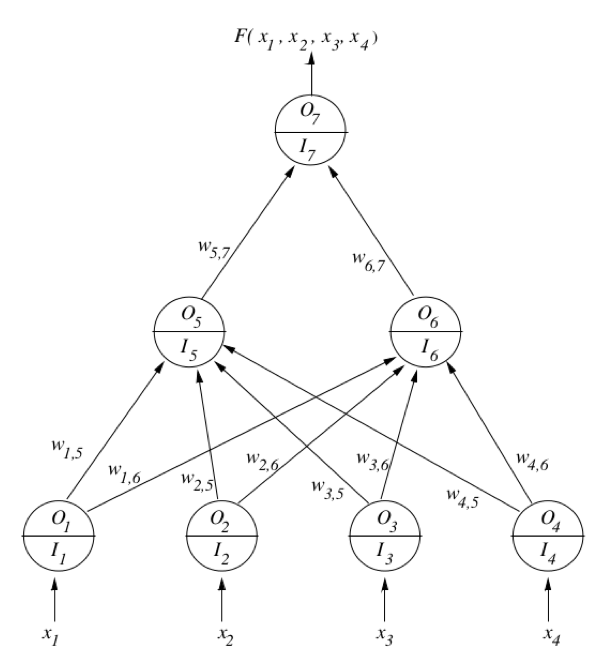
\includegraphics[width=8cm]{neural.png}
\caption{Given neural network structure. It consists in four input nodes, two hidden nodes and one exit node. With ten weights and cero bias parameters. In each node the activation function is a sigmoid function.\label{neural}}
\end{center}
\end{figure}

we can write the output function as

\begin{equation}
\begin{aligned}\label{eq1}
F(x) = \sigma_1(&\sigma_{21}(\sigma_{31}(x)\cdot I_{1,4} \cdot \hat{w} )\cdot I_{9} \cdot \hat{w}+\\
&\sigma_{22}(\sigma_{32}(x)\cdot I_{5,8} \cdot \hat{w} )\cdot I_{10} \cdot \hat{w})\\
\end{aligned}
\end{equation}

with 
\begin{equation}
\begin{aligned}
\sigma_i&=\frac{1}{1+e^{-x}}
\end{aligned}
\end{equation}
the sigmoid function\footnote{Here the subscript $i$ labels the correspondant sigmoid function}
\begin{equation}
\begin{aligned}
\hat{w}^T = (&w_{1,5},w_{2,5},w_{3,5},w_{4,5},\\
&w_{1,6},w_{2,6},w_{3,6},w_{4,6},\\
&w_{5,7},w_{6,7})
\end{aligned}
\end{equation}
the ordered weight vector\footnote{It is more convenient to treat $w$ as a vector rather than an incomplete matrix or another extructure such as a dictionary}, and 
$I_{i,j}$\footnote{This complicated matrix is constructed in such way in order that the product $I_{i,j}\cdot\hat{w} $ is a $(j-i+1)$ vector with the entries of $\hat{w}$ from $i$ to $j$ that is a matrix which selects the desired entries of $\hat{w}$} is a matrix of dimension $(4,10)$ which entries from column $i$ to  $j$ are an identity matrix and the other entries are zero e.g. 
\begin{equation}
\begin{aligned}
I_{5,8} = 
&\left(\begin{matrix}
0 &  0  & \ldots & 0\\
0  &  0 & \ldots & 0\\
\vdots & \vdots & \ddots & \vdots\\
0  &   0       &\ldots & 0
\end{matrix} \right)\, \vline \, 
&\left(\begin{matrix}
1&  0  & \ldots & 0\\
0  &  1 & \ldots & 0\\
\vdots & \vdots & \ddots & \vdots\\
0  &   0       &\ldots & 1
\end{matrix}\right)
\, \vline \,
&\left(\begin{matrix}
0 &  0  \\
0  &  0 \\
\vdots & \vdots \\
0  &   0 
\end{matrix} \right)
\end{aligned}
\end{equation}
and $I_j$\footnote{Similarly this vector selects the $j$-th entrie of $\hat{w}$} is a vector of dimension (10) which $j$-th entrie is one and the others are zero, e.g. 
\begin{equation}
\begin{aligned}
I_9^T&=\left(0,0,\cdots,0,1,0\right).
\end{aligned}
\end{equation}

We want to find a set of $\hat{w}^*$ such that 
\begin{equation}
\begin{aligned}
F(x)\rightarrow y && \forall\, x \in \mathbb{R}^4. 
\end{aligned}
\end{equation}

Thus we can define the optimization\footnote{Despite the fact that there exists several particular methods to solve neural networks (e.g. Backpropagation) we chose to use nonlinear optimization of a cost function in order to put in practice the concepts of this class } problem to be solved:

\begin{prob}\footnote{Non linear unconstrained neural network optimization}
Find $\hat{w}^*$ such that 
\begin{equation}
\begin{aligned} \label{problem1}
\min_{\hat{w}}\sum_{i=1}^p d(F_i(x;\hat{w})-y_i)
\end{aligned}
\end{equation}
\end{prob}

with $d(\cdot)$ a cost function\footnote{At first we tried with the squared euclidian distance function in a gradient descent with momentum implementation, finding convergence to  $F(x) = 0.5$ which is not desired. Thus we designed the funcion described above}. 

Since $y\in\{0,1\}$ we may ask $d$ to have this desired properties:

Let $e=F(x)-y$ then we ask for $d$:
$$\lim_{x\rightarrow-1} d(e)=\lim_{x\rightarrow 1} d(e)=+\infty$$ and 
$$f(0)=0=\arg\min _{e} d(e)$$
and since we need to find the $\nabla d(e)$ we ask $d$ to be differentiable thus continuous. 

With this in mind we propose the distance function 

\begin{equation}
\begin{aligned}\label{eq2}
d(e)=\frac{1}{1+e}+\frac{1}{1-e}-2
\end{aligned}
\end{equation}

\begin{figure}[!ht]
\begin{center}
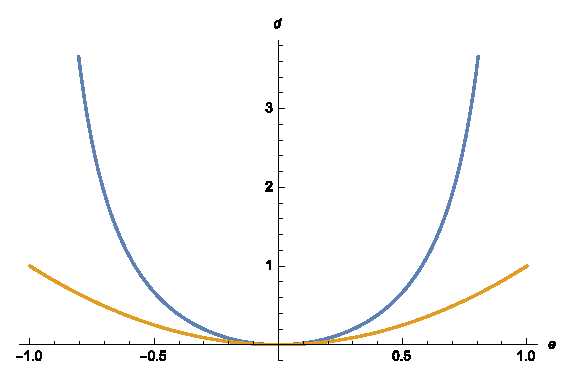
\includegraphics[width=7cm]{d.eps}
\caption{Graph of the function in equation \ref{eq2} (blue) in comparation with the squared euclidean distance (SED), (orange). The proposed function bounded in the interval (-1,1) penalices the maximum error ($\pm 1$) with infinite cost, the SED is more permisive with big differences. It holds the properties asked and is differentiable in $(-1,1)$ }
\end{center}
\end{figure}

Now, we propose to do gradient descent with a non linear solver in order to find the global minima. Thus we need to find the gradient explicitly:

\begin{equation}
\begin{aligned} \label{gradient}
\nabla_{\hat{w}_i}d(e) =& \frac{4 e}{(e^2-1)^2}\sigma_1(\cdot)(1-\sigma_1(\cdot))\\
&\sigma_{21}(\cdot)(1-\sigma_{21}(\cdot))\cdot I_9 \cdot \hat{w} \\
&\sigma_{31}(I_i\cdot x) \\ &&\text{for  } i=1,2,3,4\\
\nabla_{\hat{w}_i}d(e) =& \frac{4 e}{(e^2-1)^2}\sigma_1(\cdot)(1-\sigma_1(\cdot))\\
&\sigma_{22}(\cdot)(1-\sigma_{22}(\cdot))\cdot I_{10} \cdot \hat{w} \\
&\sigma_{32}(I_{i-4}\cdot x) \\ &&\text{for  } i=5,6,7,8\\
\nabla_{\hat{w}_i}d(e) =& \frac{4 e}{(e^2-1)^2}\sigma_1(\cdot)(1-\sigma_1(\cdot))\\
&\sigma_{2(i-8)}(\cdot)\\ &&\text{for  } i=9,10\\
\end{aligned}
\end{equation}

Recall: $\nabla_x \sigma(g(x)) = \sigma(g(x))(1-\sigma(g(x)))g'(x)$.

After finding $\hat{w}^*$ solution of the problem (\ref{problem1}) and using it in expression (\ref{eq1}) we need to apply the threshold function as follows: 

\begin{equation}
\begin{aligned}\label{pred}
\hat{F}(x)&=\begin{cases} 
      1 & F(x)\geq 0.5 \\
      0 & F(x) < 0.5 
   \end{cases}
\end{aligned}
\end{equation}

Then we can use expressions (\ref{problem1}) for the objective function, (\ref{gradient}) for the gradient and  (\ref{pred}) for the predicted value, to find the solution of the problem.

 

\section{Implementation}

The random values were supplied using the provided binary executable \texttt{genxndat} with seed \texttt{26071991}


With this in mind we chose to use the nonlinear unconstrained optimization solver of \texttt{MATLAB 7.12.0.635 (R2011a)} to solve the problem. The code used is as follows in the section \ref{code} 

\section{Tests and results}
To determine the error of prediction we first want to obtain the optimal training set size. We will evaluate the sum of the number of false positives plus the number of false negatives and divide by the size of the training set. In this particular case this reduces to:

\begin{equation}
\begin{aligned}
\epsilon&=\frac{1}{p}\sum_{i=1}^p |\hat{e}_i|\\
&=\frac{1}{p}\sum_{i=1}^p|\hat{F}_i(x)-y_i|
\end{aligned}
\end{equation}

We evaluated\footnote{That is, the mean of the error described with incertainty equal to the standard deviation of the error} $\bar{\epsilon}\pm \frac{\sigma_\epsilon}{2}$ for a 10 batch test in each order of magnitude of $p$ from 1 to 1,000\footnote{After $10^4$ observations the computation takes too much time.}. Exhibiting the results in figure \ref{batch}.

\begin{figure}[!ht]
\begin{center} \label{batch}
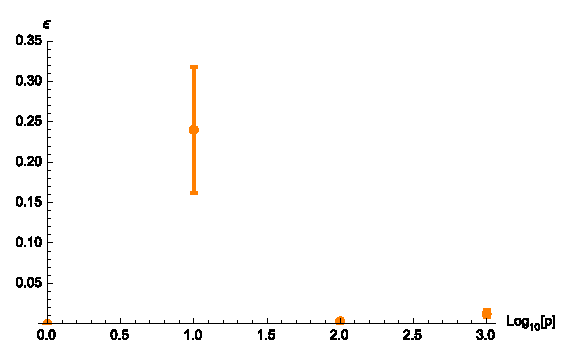
\includegraphics[width=7cm]{eps.eps}
\caption{Normalized absolute error for diferent training set sizes. For sample size $10^0$ the error es 0 in 10 tries in a row. While with a sample size of $10^1$ the error grows to $24\%\pm 7.8$. With $10^2$ training observations we get $0.30\%\pm 0.24$ but with $10^3$ the error grows again to $1.24\%\pm 0.44$.  }
\end{center}
\end{figure}

Having observed this, we decided to train the weights with a sample size of 100 observations and test the accuracy with the 1,000 sample size. Thus instead of using the Pareto approach\footnote{Train with 80\% of the set and test with 20\%} we adopt a more ambitious goal of training with just $10\%$ of the set.

\subsection{Training}
The output of the program after 90 iterations:

Initial random weights and final weights
\begin{equation}
\begin{aligned}
\hat{w}_0= \left(
\begin{array}{r}
0,352\\
-0,144\\
-0,260\\
0,911\\
2,306\\
0,847\\
0,642\\
0,004\\
0,129\\
0,581
\end{array}
\right)
&&\hat{w}^*= \left(
\begin{array}{r}
-0,750\\
-0,940\\
-0,986\\
-0,892\\
4803,786\\
4565,815\\
4122,838\\
4515,028\\
-16840,135\\
1662,110
\end{array}
\right)
\end{aligned}
\end{equation}

Convergence graph in figure \ref{convergence}. 

The error rate is equal to $\epsilon=0\%$

\begin{figure}[!ht]
\begin{center}
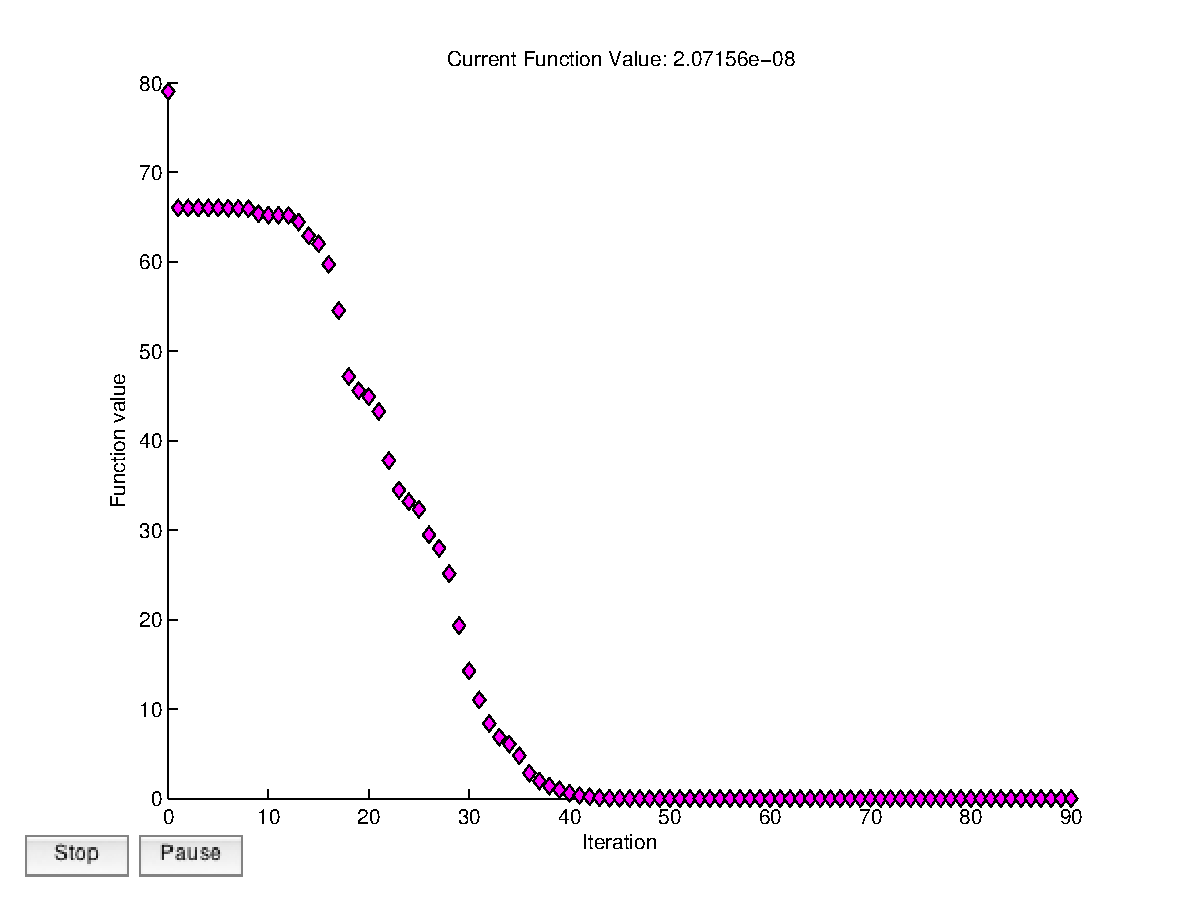
\includegraphics[width=8.5cm]{conv.eps}
\caption{\label{convergence}Value of the objetive function (\ref{problem1}) through the iterations.}
\end{center}
\end{figure}

\subsection{Testing}
We know that the \emph{true} relation between input vectors $x$ and labels $y$ is described by

\begin{equation}
\begin{aligned}
y&=\begin{cases} 
1 & \text{if  }  \sum_{i=1}^4x_i >2\\ 
0 & \text{if  }  \sum_{i=1}^4x_i \leq2
\end{cases}
\end{aligned}
\end{equation}

With this in mind we computed the $$\sum_{i=1}^4x_i$$ and compared $$\hat{e}=\hat{F}_i(x)-y_i$$ Taking the weights learned $\hat{w}^*$ but with the $10^3$ test set. 

The prediction got an error rate of $\epsilon=2.9\%$. If we graph the pairs $$\left(\sum_{i=1}^4x_i,\hat{e}\right)$$ we get figure \ref{confusion}

\begin{figure}[!ht]
\begin{center}
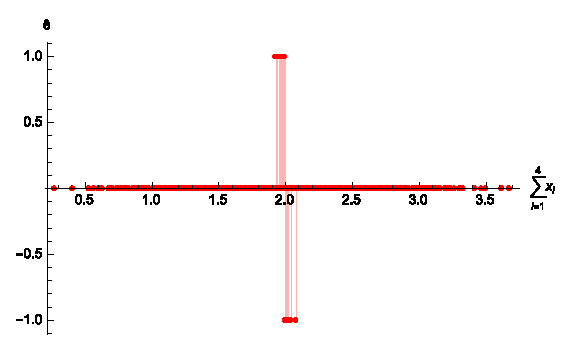
\includegraphics[width=8.5cm]{e.eps}
\caption{Graphical representation of the points that get missclassified in the test set. we observe clearly that they are near the change point.
\label{confusion}}
\end{center}
\end{figure}

In fact if we take the missclassified points minus two and see their ditribution we observe figure \ref{dist}

\begin{figure}[!ht]
\begin{center}
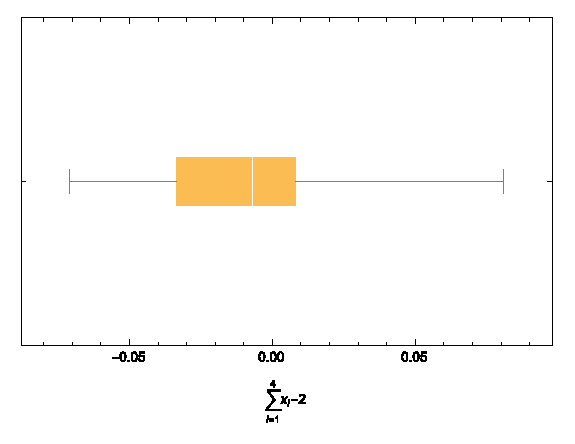
\includegraphics[width=8.5cm]{dist.eps}
\caption{Taking the distance of missclassified points to the change point we observe that they are at most at $0.081$ distance in median at $-0.007$ and in average at $-0.0103$, that is, very close\label{dist}}
\end{center}
\end{figure}

\section{Conclusions}

\begin{enumerate}
\item Giving a special treatment to the problem, we were able to pose an unconstrained non linear optimization problem and we found a solution using a proprietary solver 
\item Evaluating the test sample size, we were able to reduce computation time and over-fitting issues.
\item The training set achieved $0\%$ error while the test set achieved $2.9\%$ even though the training set is just $10\%$ portion of the test set.
\item The false positive and false positive points correspond entirely of the region around the transition of label. That is, the neural network encounters problem classifying points near the transition point.
\end{enumerate}

\newpage
.
\newpage

\section{Implementation Code}\label{code}
\lstset{
language={matlab},
basicstyle=\tiny,
numbers=left,
numberstyle=\tiny,
numbersep=5pt, 
showspaces=false,
showstringspaces=false,
showtabs=False,
frame=false,
%tabsize=.5,
keywordstyle=\bfseries\color{green!40!black},          % keyword style
 commentstyle=\itshape\color{purple!40!black},       % comment style
 identifierstyle=\color{blue},
  stringstyle=\color{orange},
basicstyle=\ttfamily,
captionpos=b}
\lstdefinestyle{matlab}{
language={matlab},
basicstyle=\tiny,
numbers=right,
numberstyle=\tiny,
numbersep=5pt, 
showspaces=false,
showstringspaces=false,
showtabs=False,
frame=single,
tabsize=.5,
keywordstyle=\bfseries\color{green!40!black},          % keyword style
 commentstyle=\itshape\color{purple!40!black},       % comment style
 identifierstyle=\color{blue},
  stringstyle=\color{orange},
basicstyle=\ttfamily,
captionpos=b,
title=\lstname
}

\lstinputlisting[language=matlab,basicstyle=\small,numberstyle=\tiny]{code2.m} \vspace{0.1cm}


\end{document}